\documentclass[10pt]{article}
\usepackage{../../local}
\urlstyle{same}

\newcommand{\classcode}{EE 120}
\newcommand{\classname}{Signals and Systems}
\renewcommand{\maketitle}{%
\hrule height4pt
\large{Eric Du \hfill \classcode}
\newline
\large{Lecture Notes} \Large{\hfill \classname \hfill} \large{Chunlei Liu}
\hrule height4pt \vskip .7em
\small{Header styling inspired by CS 70: \url{https://www.eecs70.org/}}
\normalsize
}
\linespread{1.1}

\newcommand{\question}[1]{\textcolor{red}{#1}}
\newcommand{\answer}[1]{\textcolor{green!80!black!}{#1}}
\renewcommand{\comment}[1]{\textcolor{blue!50}{#1}}

\newcommand{\corr}{\mathrm{corr}}
\begin{document}
	\maketitle
	\section{Introduction}
\begin{itemize}
	\item Let's go back to 1974, e
	\item No classical theory permits this gradual energy loss, except in General Relativity!
	\item Speaking of General relativity, one thing it predicted was the present of gravitational waves (GW), and 
		this was where the lost energy was going. Specifically, we can calculate its power:
		\[
		P = -\frac{2}{5}\frac{G^{4}M^{5}}{R^{5}c^{5}}
		\] 
	\item We commonly think of \( G = 6.67 \times 10^{-11}\), but later in the course we're going to work in units 
		where \( G = 1 \), to simplify things. 
	\item In electrodynamics, an charge \( q \) that experiences an acceleration also emits electromagnetic waves. This
		is called synchrotron radiation:
		\[
			P = -\frac{2}{3} \left( \frac{q^2}{4\pi \epsilon_0} \right) \frac{a^2}{c^3}
		\] 
		To get a sense of the scale of this power, the amount that our solar system is losing due to the sun and 
		Jupiter is around 200 W. But Hudson and Taylor found a power of \( P = -7 \cdot 10^{34} \) W!
	\item In 1983, they measured this, in 1993 they won the Nobel prize for their indirect detection of 
		gravitational waves. In 2015, LIGO detected these waves directly, and found a power 
		\( P = 3.6 \times 10^{49} \) W. In 2017, they won the Nobel prize for this discovery. 
\end{itemize}
\subsection{Why General Relativity?}
\begin{itemize}
	\item In Newton's gravity, we have the equation \( \vec F_i = \dv[2]{\vec r_i}{t} \), and for universal 
		gravitation, we had:
		\[
		\vec F_i = \sum_{j\neq i}\frac{G m_i m_j}{|\vec r_i - \vec r_j|^3}(\vec r_j - \vec r_i)
		\] 
		\comment{Note that it's only formatted like this so that we can talk about vectors.}
	\item One problem with this interpretation is that things are instantaneous: this is an issue because objects
		don't react instantaneously to changes (information 
		can't travel faster than the speed of light), which Newton's equations seem to imply. 

		We can say the same about Coulomb's law: and the solution there was to replace the notion of a force 
		with \textit{fields}. Now, the force can be written as: 
		\[
		\vec F_i = q(\vec E + \frac{1}{c}\vec v \times \vec B)
		\] 
		\comment{We'll use Gaussian units, mainly because \( \vec E \) and \( \vec B \) now have the 
		same units. With this,
		\begin{align*}
			\vec \div E &= 4 \pi \rho \\
			\vec \div B &=  0 \\
			\vec \curl E &= -\frac{1}{c}\pdv{\vec B}{t}\\
			\vec \curl B &= \frac{1}{c}\pdv{\vec E}{t} + \frac{4\pi}{c}\vec J 
		\end{align*}		}
		So the question then becomes: why didn't we do this for Gravitation? Well, this is a thing, but it's 
		only an approximation. 
	\item Let's talk about energy conservation: in E\&M, the energy is written as:
		\[
		\mathcal E = \frac{1}{8\pi}\int (\vec E^2 + \vec B ^2) dv + \sum_i k_i
		\] 
		What happens when we change the sign on everything to accomodate for gravitation? Then, we introduce instability 
		into the system! 
\end{itemize}
	
	\section{Divide and Conquer I, Asymptotics}
\begin{itemize}
	\item Last time, we talked about the motivations for studying algorithms: designing ways to solve problems efficiently. 
	\item We also talked about addition and multiplication, and the latter in particular we saw two algorithms for it, but 
		couldn't break the \( O(n^2) \) runtime. Today, we'll try to beat this.
\end{itemize}

\subsection{Karatsuba's Algorithm}
\begin{itemize}
	\item The main issue we ran into with the divide and conquer algorithm is that when we broke a problem down, we didn't 
		actually simplify our life at all -- we just created subproblmes for ourselves. What if we can create 
		fewer than 4 subproblems? This is the key idea with divide and conquer: if we can use the results of subproblems 
		to simplify computation at a given layer, we can generate an overall speedup.
	\item In Karatsuba's case, if we can write the term \( \text{P2} + \text{P3} \) in terms of P1 and P4, then we can 
		simplify the number of computations needed. 
	\item Karatsuba's trick is as follows: let's compute only three things:
		\begin{itemize}
			\item Q1: \( a \times c \) 
			\item Q2: \( b \times d \) 
			\item Q3: \( (a + b)(c + d) \)
		\end{itemize}
		Then, the idea is that the middle term \( \text{P2} +  \text{P3} \) can be written in terms of these smaller subproblems:
		\[
		a\times d + c\times b = (a + b)(c + d) - ac - bd
		\] 
		Therefore, our multiplication now looks like:
		\begin{align*}
			x \times y &= \left( a \times 10^{n / 2} + b \right) \left( c \times 10^{n /2} + d \right) \\
					   &= \underbrace{(a \times c)}_{\text{Q1}} 10^{n} + \underbrace{(a \times d + c \times b)}_{\text{Q3} - 
					   \text{Q1} - \text{Q2}} 10^{ n / 2} + \underbrace{(b \times d)}_{\text{Q3}}
		\end{align*}
	\item With this algorithm, what is the runtime of this algorithm? The problem is almost the same, except we now only have 
		3 subproblems instead of 4. Therefore, if we employ the tree method (just as last time), then we'll see that 
		we have \( \log_2(n) \) layers, which means we have \( 3^{\log_2 n} = n^{\log_2 3} \approx n^{1.6} \), which is 
		where we get our runtime from.
		\begin{itemize}
			\item The Toom-3 algorithm mentioned last lecture also uses divide and conquer, but instead it reduces 
				9 problems into 5 subproblems, which gives a better bound. 
		\end{itemize}
	\item Note that Karatsuba's algorithm also doesn't care about the base we're working in: this works with any base. 
		Note that the factor of \( 2^{n /2} \) that will appear in the division step is also just adding zeros, but in binary! 
\end{itemize}
\subsection{Asymptotic Notations (Formally)}
\begin{itemize}
	\item Suppose an algorithm takes \( T(n) = 5n^2 + 20n \log n + 7 \) microseconds. Then, we say that \( T(n) \in O(n^2) \), or 
		also sometimes written as \( T(n) = O(n^2) \).
	\item Why do we employ this \( O(\cdot) \) notation? It's because constants like 5, 20, 7 usually depend on the computer 
		(say your computer is a year newer and has a faster CPU inside), so getting rid of these constants make comparing algorithms
		much easier. It's also often the case that the constants can be improved via some other smaller, less important 
		optimizations. 
	\item The formal definition of \( O(\cdot) \) is as follows: 

		Let \( T(n) \) and \( g(n) \) be functions of positive integers. Think of \( T(n) \) as a runtime, so it's positive and 
		increasing with \( n \) (usually). Then, we say "\( T(n) \) is  \( O(g(n)) \)" if and only if for some large enough 
		\( n \), \( T(n) \) is at most some constant multiple of \( g(n) \). Mathematically:

		There exists \( c \) and \( n_0 > 0 \) such that for all \( n \ge  n_0\), \( T(n) \le  c \cdot g(n) \). 

		Note that this \( g(n) \) also isn't unique! If a function is in \( O(n^2) \), then it's also \( O(n^3) \), and it's 
		also in \( O(2n^2) \). However, we generally ask for the simplest and the tightest bound, so while these are 
		all technically correct answers, \( O(n^2) \) is the "most correct". 
	\item As an example, we can prove that \( T(n) = 2n^2 + 2 \in O(n^2)\). Here, we can choose \( n_0 = 1 \), \( c = 4 \), 
		so that we have: 
		\[
		2n^2 + 2 \le 4n^2
		\] 
		All we have to do is prove that this inequality holds for all \( n \ge  n_0 \). We can do this via derivatives, or other 
		equivalent methods. 
	\item There's an equivalent definition for a lower bound: we say that "\( T(n) \in \Omega(g(n)) \)" if and only if 
		there exists \( c \) and \( n_0 > 0 \) such that for all \( n \ge n_0 \), \( c \cdot g(n) \le T(n) \). Note that this 
		inequality is reversed from the previous one. 

	\item To test asymptotics, one way that's particularly efficient is using limits: 
		\[
			\lim_{n \to \infty} \frac{T(n)}{g(n)} = \begin{cases}
				0 & T(n) \in O(g(n))\\
				c \in \mathbb R & T(n) \in \Theta(g(n))\\
				\infty & T(n) \in \Omega(g(n))
			\end{cases}
		\] 
	\item The asymptotics of the geometric series is quite important for runtime analysis. Take any constant \( r \) and 
		a function \( T(n) = 1 + r + r^2 + \cdot + r^{n} \). We have that:
		\[
		T(n) = \begin{cases}
			\Theta{r^{n}} & \text{if \( r > 1 \) }\\
			\Theta(1) & \text{if \( r < 1 \)}\\
			\Theta(n) & \text{if \( r = 1 \)}
		\end{cases}
		\] 
		\textit{Proof:} Recall that for a goemetric series with \( r \neq 1 \), then we have:
		\[
		1 + r + r^2 + \cdots + r^{n} = \frac{r^{n+1} - 1}{r-1}
		\] 
		For \( r > 1 \), then this right hand side roughly evalutes to \( \frac{r^{n + 1}}{r} = r^{n} \), hence the 
		\( \Theta(r^n) \) bound. For \( r < 1 \), \( r^{n + 1} \) is going to be very small, and hence \( r^{n + 1} - 1 < 0\). 
		Overall, this means 
		\[
			\frac{r^{n + 1} - 1}{r - 1} \approx \frac{1}{1 - r}
		\] 
		and since \( r \) is a constant we have \( T(n) = \Theta(1) \). For \( r = 1 \), then we have \( T(n) = n \in \Theta(n)\). 
\end{itemize}
\subsection{Formal Proof of Karatsuba's}
\begin{itemize}
	\item Now we formally look at Karatsuba's algorithm runtime. At each layer, we have 3 subproblems, each of size \( n / 2 \).  
		At every layer, we have to do a bunch of things: finding Q1, Q2, Q3, additions, and other stuff. However, all of 
		this stuff runs in \( O(n) \) time. To use a specific number, we'll say that the work is \( 20n \). Therefore, 
		we have the following formula for \( T(n) \): 
		\[
		T(n) = 3T\left( \frac{n}{2} \right)  + 20n
		\] 
		This is a \textbf{recurrence relation.} We should also have a base case: \( T(1) = O(1) \). Now, our goal is to find a 
		closed form relation to \( T(n) \). 

		Now we look at this layer by layer. At the first layer, we have 1 problem, so that has \( 20n \) units of work. At 
		the second layer, we have 2 subproblems, each of size \( n / 2 \), so we have \( 3 \times 20 \times \frac{n}{2} \) 
		amount of work from this layer. In general, we have:
		\[
		\text{work} = (\text{number of subproblems}) \times 20 \times (\text{subproblem size})
		\] 
		This translates into the equation
		\[
		3^{t} \cdot 20 \left( \frac{n}{2^{t}} \right) 
		\] 
		We now need to sum this for all \( t \), so we have:
		\begin{align*}
			T(n) &= \sum_{t = 0}^{\log_2 n}3^{t} \cdot 20 \cdot \left( \frac{n}{2^{t}} \right) \\
			&= 20n \sum \left( \frac{3}{2} \right)^{t} 
		\end{align*}
		Now recall the geometric series we had from earlier: since \( r = \frac{3}{2}> 1 \), then the summation 
		is \( \Theta((3 / 2)^{\log_2 n}) \), so overall:
		\[
		T(n) = 20n \left( \Theta\left( \frac{3}{2} \right)^{\log(n)} \right) = 
		O\left(n \left( \frac{3}{2} \right) ^{\log 3 - \log 2}\right) = O(n^{\log 3}) = O(n^{1.6})
		\] 
\end{itemize}
\subsection{The Master Theorem}
\begin{itemize}
	\item The tree method is useful, but slightly annoying to deal with sometimes. There's a theorem, called the Master Theorem, 
		that tells us the runtime of \( T(n) \), if we have a recurrence relation of the following form:
		\[
		T(n) = a \cdot T\left( \frac{n}{b} \right) + O(n^{d})
		\] 
		Then, we have:
		\[
		T(n) = \begin{cases}
			O(n^{d}) & \text{if \( a < b^{d} \)}\\
			O(n^{d} \log(n)) & \text{if \( a = b^{d} \)}\\
			O(n^{\log_b(a)}) & \text{if \( a > b^{d} \)}
		\end{cases}
		\] 
	\item The Master Theorem only tells us the runtime given this very specific recurrence relation. In fact, as you'll notice 
		with the \( O(n^{d}) \) term, it only works if the work at every step is polynomial. Also, if \( n / b \) is not an 
		integer, we can force it to be an integer by enforcing a recurrence relation of the form:
		\[
		T(n) = a \cdot T\left( \left\lceil \frac{n}{b} \right\rceil  \right) + O(n^{d})
		\] 
		Loosely, this is because constants don't matter, so small shifts (of less than 1) in the subproblem size doesn't really 
		change the recurrence relation at all. 
\end{itemize}


	\section{Characterization Continued}
\subsection{Step Response}
\begin{itemize}
	\item The step response function is the function \( y_{\text{step}}(t) \) when a step function 
		\( u(t) \) is fed into the system. In discrete-time: we feed \( u[n] \) into the system, and get 
		\( y_{\text{step}}[n] \) as an output.
	\item For instance, for the moving average filter defined earlier, we have the following result:
		\begin{center}
			\begin{tabular}{c|c}
				\( n \) &  \( y_{\text{step}}[n] \)\\
				\hline 
				-2 & 0\\
				-1 & 1/3\\
				0 & 2/3\\
				1 & 1\\
				2 & 1
			\end{tabular}
		\end{center}
		Note that this resembles a ramp function, and is called a ramp-step function.
	\item \textbf{Harmonic Response:} The harmonic response is the response by the system when presented with 
		a harmonic function, of the form \( Ae^{i \omega t}\). 

		In discrete time, we feed in \( Ae^{i \omega n} \) where \( n \) is an integer. 
	\item For the moving average filter, let's write out \( y[n] \) :
		\begin{align*}
			y[n] &= \frac{1}{3}\left(Ae^{i \omega (n - 1)} + Ae^{i \omega n} + Ae^{i \omega (n + 1)}\right)\\
			&= \frac{1}{3}\left( e^{-i \omega} + 1 + e^{i \omega} \right)  \\
			&= \frac{1}{3}(2 \cos \omega + 1) Ae^{i \omega n} \\
		\end{align*}
		The interesting thing here is that when given a harmonic function, the system response just scales the signal 
		by a constant amount!
\end{itemize}
\subsection{LCCDE} 
\begin{itemize}
	\item In this class, we will deal with lots of differential equations, so it's going to be very useful to 
		look at their form, and how to solve them.   
	\item There are two solutions to any differential equation: 
		\begin{itemize}
			\item \textbf{Particular Solution:} \( y_p(t) \) is called a particular solution if it satisfies:
				\[
					\sum_{k = 0}^{N}a_k \dv[k]{y_p(t)}{t} = \sum_{k = 0}^{N}b_k \dv[k]{x(t)}{t}
				\] 
			\item \textbf{Homogeneous Solution:} \( y_h(t) \) is called a homogeneous solution if it satisfies:  
				\[
						\sum_{k = 0}^{N}a_k \dv[k]{y_p(t)}{t} =	0
				\] 
		\end{itemize}
	\item In general, the solution will be a linear combination of the two: 
		\[
		y(t) = y_p(T) + ay_h(t)
		\] 
		the value of \( a \) is generally going to be given by some initial condition. 
	\item For the homogeneous solution, an ansats of the form \( Ae^{st} \) where \( s \) is an undetermined constant 
		will solve the differental equation. We can then determine the value of \( s \) by solving the resulting 
		polynomial.

		To determine the value of \( A \), these are determined by the initial conditions, and depending on the 
		number of initial conditions given, that would correspond directly to the number of distinct values of \( A \). 
\end{itemize}


	\section{Polynomial Multiplication}
\begin{itemize}
	\item Earlier, we talked about multiplying numbers and also matrices quickly. Today, we'll talk about manipulating polynomials.
	\item Given two polynomials \( p(x) \) and \( q(x) \), what are the fastest algorithms that add and 
		multiply the two polynomials together?
\end{itemize}
\subsection{Representing Polynoimals}
\begin{itemize}
	\item Typically, we'd write a degree \( n-1 \) polynomial as 
		\( p(x) = p_0 + p_1x + p_2x^2 + \cdots + p_{n-1}x^{n-1} \). This is called
		the \textbf{coefficient representation}, represented by an array of numbers \( (p_0, p_1, \cdots, p_{n-1}) \). 
		Note that \( p_i \) 
		 are \textit{real numbers}, not necessarily integers.  
	 \item We will think of \( n \) as being very large, say \( n = 10^{10} \), while thinking that \( p_0, \cdots, p_{n-1} \)
		 to be very small. So we'll imagine that all these arithmetic operations are going to take \( O(1) \) time.  
	 \item Goal: measure runtime as a function of \( n \), not on the coefficients themselves.    
\end{itemize}
\subsection{Adding Polynomials}
\begin{itemize}
	\item Given two polynomials \( p(x) \) and \( q(x) \), we want to output \( r(x) = p(x) + q(x) \), in its coefficient 
		representation. 
	\item How fast can we do this? To find the coefficients of \( r(x) \), we just add \( r_i = p_i + q_i \), and since each 
		takes constant time, there are \( n \) additions, hence \( O(n) \). 
	\item This is like adding integers, but even simpler, since there is no carry over term!
\end{itemize}
\subsection{Evaluating Polynomials}
\begin{itemize}
	\item Given an input \( p(x) = p_0 + p_1x + p_2x^2 + \cdots + p_{n-1}x^{n-1} \), and a real number \( \alpha \in \mathbb R \). 
	\item We want to output \( p(\alpha) = p_0 + p_1\alpha + p_2\alpha^2 + \cdots + p_{n-1}\alpha ^{n-1} \in \mathbb R \). 
	\item How fast can we do this? There are three algorithms that take \( O(n^2) \), \( O(n \log n) \), and \( O(n) \) 
		respectively. We'll first take a look at the \( O(n^2) \) and the \( O(n) \) ones. 
		\begin{itemize}
			\item Algorithm 1: We compute the terms individually and add them together: 
				\begin{align*}
					&\phantom{+a} p_0 & \text{0 multiplications}\\
					&+ p_1 \cdot \alpha & \text{1 multiplication}\\
					&+ p_2 \cdot \alpha \cdot \alpha & \text{2 multiplications}\\
					&+ p_3 \cdot \alpha \cdot \alpha \cdot \alpha & \text{3 multiplications}\\
					&\vdots\\
					&+ p_{n-1} \cdot \alpha \cdot \alpha \cdots \alpha & \text{\( n-1 \) multiplications}\\
					&\rule{4cm}{0.6pt}&\\
					&p(\alpha) & \text{\( O(n^2) \) multiplications}
				\end{align*}
			Notice the repeated computation we have here: when we compute \( \alpha^3 \), we don't actually need to multiply
				\( \alpha \) three times, since we've already computed \( \alpha^2 \) in the previous step. 
			\item Algorithm 2: Initialize an array \( A \), and set \( A[i] = \alpha \cdot A[i-1] \) for each 
				\( i = 1, 2, \dots \). Therefore,  \( A = [1, \alpha, \alpha^2 , \alpha^3, \cdots] \). So every step here 
				takes 1 multiplication, so to compute the whole array \( A \) takes \( O(n) \) steps. Now, if we were to evaluate 
				now:
				\begin{align*}
					&\phantom{+a} p_0 \cdot A[0]& \text{1 multiplication}\\
					&+ p_1 \cdot A[1]& \text{1 multiplication}\\
					&+ p_2 \cdot A[2] & \text{1 multiplication}\\
					&+ p_3 \cdot A[3] & \text{1 multiplication}\\
					&\vdots\\
					&+ p_{n-1} \cdot A[n-1]& \text{1 multiplication}\\
					&\rule{4cm}{0.6pt}&\\
					&p(\alpha) & \text{\( O(n) \) multiplications}
				\end{align*}
				Therefore, this will take \( O(n) \) total steps, hence an \( O(n) \) runtime.  

				\comment{Note here that \( n \) (the problem size) refers to the length of the polynomial, and not the size 
					of the coefficients \( p_i \). We assume these to be small for our analysis, but this is not true in practice, 
				and these computations will add up.}
		\end{itemize}
\end{itemize}
\subsection{Multiplying Polynomials}
\begin{itemize}
	\item Given two polynomials \( p(x) \) and \( q(x) \), we want to output \( p(x) \cdot q(x) \). For instance, \( p(x) = 
		(7 - 5x), q(x) = (1 + 3x + 2x^2)\). If we were to do this by hand, we find that \( p(x) \cdot q(x) = 
		7 + 26x + 29x^2 + 10x^3\).
	\item How fast can we do this? \( O(n^2) \). This is because for every coefficient in \( p \) we need to perform 
		\( n \) multiplications (one for every coefficient in \( q \)), and since \( p \) has \( n \) coefficients then there are 
		\( n^2 \) total multiplications. Hence, the runtime is \( O(n^2) \). 

		Note also that in doing so, we also increase the degree of the product, with it being a degree \( 2n-2 \) polynomial.

		Our goal for the rest of today's lecture is to improve this to \( O(n \log n)  \) time.  
	\item To do this, we use the fact that \( n \) points determine a degree \( n-1 \) polynomial (recall this from 
		cs70 notes) In other words, 
		if \( p(x) \) is degree 1, then 2 points suffice; if \( p(x) \) is degree 2, then we need 3 points, and so on.
	\item This is useful because instead of representing polynomials 
		by their coefficients, we can instead represent them by values given certain inputs. So given some points \( \alpha_1, 
		\alpha_2, \dots, \alpha_m \in \mathbb R\), the value representation of \( p(x) \) is given by 
		\( (p(\alpha_1), p(\alpha_2), \dots, p(\alpha_m)) \). 
	\item Using the previous fact, as long as \( m \ge n  \), then the polynomial is uniquely determined. For us, 
		a typical choice of \( m \) is \( m = O(n) \). 
\end{itemize}
\subsubsection{Adding and Multiplying with Value Representation}
\begin{itemize}
	\item Given two polynomials in their \textit{value representation}, how would we add these two polynomials together? We can 
		just add these two values together, and output \( (p(\alpha_1) + q(\alpha_1), \dots, p(\alpha_m) + q(\alpha_m) \). This 
		takes \( O(n) \) time. 
	\item For multiplication, we output the product of the values: \( (p(\alpha_1) \cdot q(\alpha_1), \dots, 
		p(\alpha_m) \cdot q(\alpha_m) \). This is also \( O(n) \). However, one thing to note with multiplication is because
		the degree of the product changes, we need \( m \ge 2n-1 \) in order for the result to uniquely specify the product. 
	\item The takeaway is that multiplication is much faster in the value representation compared to the coefficient representation!
\end{itemize}
\subsection{Fast Polynomial Multiplication}
\begin{itemize}
	\item The last section motivates a scheme where we multiply polynomials using their value representation rather than their 
		coefficient representation. Therefore, we need the following scheme:
		\begin{center}
			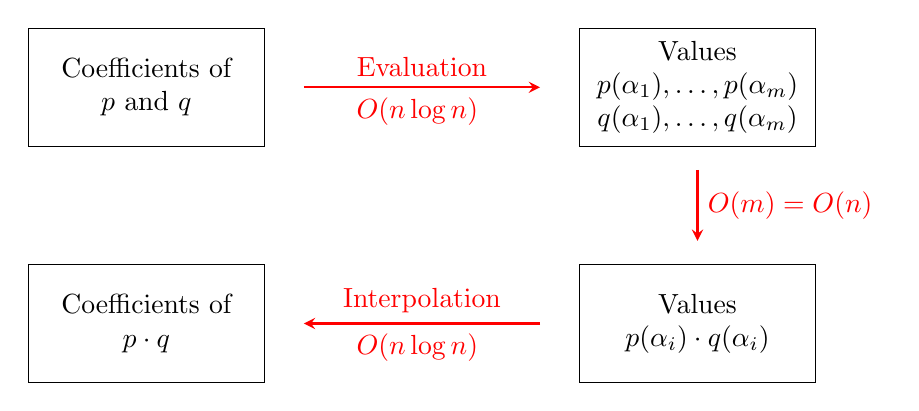
\begin{tikzpicture}[every text node part/.style={align=center}]
				\foreach \x in {0, 7}
				\foreach \y in {0, 3}
				{
					\draw (\x, \y) -- (\x+3, \y) -- (\x+3, \y+1.5) -- (\x, \y+1.5) -- cycle;
				}
				\draw node at (1.5, 0.75) {Coefficients of \\ \( p \cdot q \)};
				\draw node at (1.5, 3.75) {Coefficients of \\ \( p \) and \( q \) };
				\draw node at (8.5, 0.75) {Values \\ \( p(\alpha_i) \cdot q(\alpha_i) \) };
				\draw node at (8.5, 3.75) {Values \\ \( p(\alpha_1), \dots, p(\alpha_m) \) \\ \( q(\alpha_1), \dots, q(\alpha_m) \) };
				\draw[-stealth, red, thick] (3.5, 3.75) --node[midway, above] {Evaluation} node[midway, below] 
					{\( O(n \log n) \) } (6.5, 3.75); 
				\draw[-stealth, red, thick] (8.5, 2.7) -- node[midway, right] {\( O(m) = O(n) \) } (8.5, 1.8);
				\draw[-stealth, red, thick] (6.5, 0.75) -- node[midway, above] {Interpolation} node[midway, below] 
					{\( O(n \log n) \) } (3.5, 0.75);
			\end{tikzpicture}
		\end{center}
		If we can do this whole sequence, then that gives us an efficient multiplication algorithm. However, the evaluation step 
		still takes \( O(m \cdot n) = O(n^2) \) time, so how can we possibly get this down to \( O(n \log n) \)? The secret 
		lies in how we pick \( \alpha_1, \dots, \alpha_m \) -- it is possible to pick them in such a way that the evaluation 
		step takes \( O(n \log n) \) time. Same goes for interpolation. 

		How do we pick \( \alpha_1, \dots, \alpha_m \)? We use complex numbers!
\end{itemize}

\subsection{Complex Numbers}
\begin{itemize}
	\item A complex number is any number of the form \( a + bi \), where \( i = \sqrt{-1}  \). \( a \) represents the real part, and 
		\( b \) represents the imaginary part of the number. We can add complex numbers:
		\[
			(1 + 2i) + (3 + 4i) = (1 + 3) + (2 + 4)i = 4 + 6i
		\] 
		so the real parts add and the imaginary part also adds. To multiply:
		\[
			(1 + 2i) \cdot (3 + 4i) = 1 \cdot 3 + 1 \cdot 4i + 2i \cdot 3 + 2i \cdot 4i = 3 + 10i - 8 = -5 + 10i
		\] 
		Recall that since \( i = \sqrt{-1}  \), then  \( i^2 = -1 \). 
	\item We can also represent complex numbers on the complex plane. A number \( a + bi \) corresponds to  \( (a, b) \) on the 
		complex plane. We can also represent it using polar coordinates, using a radius \( r \) and an angle \( \theta \)
		\begin{center}
			\begin{tikzpicture}
				\draw (-3, 0) -- (3, 0) node[above] {real};
				\draw (0, -3) -- (0, 3) node[above right] {imaginary};
				\draw[red] (0, 0) -- node[midway, above] {\( r \) } (1.8, 1.4) node[above right, black] {\( (a, b) \) }; 
				\filldraw[red] (1.8, 1.4) circle (2pt); 
				\draw[red] (1, 0) arc (0:37.87:1) node[midway, right]{\( \theta \) };
			\end{tikzpicture}
		\end{center}
		With this construction, we can relate polar to cartesian with the relations
		\begin{align*}
			a &= r\cos\theta \\
			b&= r \sin \theta 
		\end{align*}
		For today, we'll only consider points with \( r = 1 \). This means that we basically forget about \( r \), and only 
		worry about \( \theta \). So with \( r = 1 \), then we have:
		\begin{align*}
			a &=  \cos \theta \\
			b &=  \sin \theta 
		\end{align*}
		And since \( r = 1 \), we'll be dealing with points on the \textbf{unit circle}.
	\item Consider two complex numbers, the first specified by \( \theta_1 \), and the other specified by \( \theta_2 \) (both 
		having \( r = 1 \) ). Then, we define the product of the two to be specified by \( \theta_1 + \theta_2 \). To multiply, 
		we just add the angles.
\end{itemize}
\subsubsection{Roots of Unity}
\begin{itemize}
	\item The \( n \)-th root of unity is a solution to the equation \( x^{n} = 1 \). So the second roots of uhnity are solutions 
		to the equation \( x^2 = 1 \), which are \( \pm 1 \). The 4-th roots of unity are solutions to \( x^{4} = 1 \), 
		which are \( \{1, -1, i, -i\}  \). 
	\item In general, the \( n \)-th roots of unity will have \( n \) distinct solutions. 
	\item Graphically, the \( n \)-th roots of unity correspond to \( n \) equally spaced points placed on the unit circle.   
	\item When we talk about the roots of unity, we will use \( \omega_0 \) through \( \omega_{n-1} \) to label them. In particular, 
		we'll focus on \( \omega_1 \).
		\begin{itemize}
			\item Note that \( \omega_1 \) always sits at an angle of \( \frac{2\pi}{n} \) for the \( n \)-th roots of unity, due 
				to the even spacing.
			\item Note that \( \omega_2 = \omega_1 \cdot \omega_1 \), since multiplying is equivalent to adding the angles together.
				Therefore, we have the relation that \( \omega_i = \omega_1^{i} \), which we will call the \textbf{Generator Fact}. 
		\end{itemize}
	\item So this gives us a nice formula for the \( n \)-th roots of unity: they will always sit at angles \( k\theta \), where 
		\( \theta = 2\pi / n \). As angles, this is represented as the set: \( \{\cos(k\ell) + i\sin(k\ell) | \ell= 0, 1, \dots, 
		n - 1\}  \).  
\end{itemize}
\subsubsection{Square Roots}
\begin{itemize}
	\item When we take a square root, remember that they always come in pairs of \( \pm \sqrt{a}  \). So to get the second 
		roots of unity, we find the square roots of 1, which are \(  \pm 1 \). To get the 4-th roots of unity, then we just need 
		to take the square roots of the previous roots of unity. 

		In general, if we take the square roots of the \( n \)-th root of unity, then we generate the \( 2n \)-th root of unity. 
		Conversely, if we square the roots of unity then we get the \( n / 2 \)-th roots of unity. 

		This is the magical fact that we will leverage for the following lecture: squaring the \( n \)-th roots gives us 
		the \( n / 2 \)-th roots of unity. This is not true for most numbers! For instance, squaring the set \( \{1, 3, 5, 7\}  \)
		gives \( \{1, 8, 25, 49\}  \), which still contains the same number of elements as the original set!
\end{itemize}
\subsection{Fast Polynomial Multiplication Algorithm (Preview)}
\begin{itemize}
	\item Recall the evaluation step in our polynomial multiplication: \( p \cdot q \) is degree \( 2n - 2 \), so we need 
		\( m \ge 2n - 1 \). Let \( m \) be the first power of 2 such that \( m \ge  2n - 1 \). Then, we will evaluate \( p \) 
		and \( q \) on the \( m \)-th roots of unity in time \( O(m \log m) = O(n \log n)\), 
		using the \textbf{Fast Fourier Transform}.  
\end{itemize}

	\section{Quantum Key Distribution}
\begin{itemize}
	\item Qubits used for communication are usually photons, which have a momentum \( \vec k \), and 
		an electric field \( E_x \) and \( E_y \) that propagates in the plane perpendicular to \( \vec k \). 
		The \( E_x \) vector is denoted as \( \ket*{v} \), and  \( E_y \) as \( \ket*{H} \), and this means that 
		the general electric field \( \overline E = \alpha \ket*{v} + \beta \ket*{H} \). 
	\item We can pass these photons thorugh polarizers, which only transmit light with specific oscillations.  
	\item So as a quantum circuit, it's written as:
		\begin{center}
			\begin{quantikz}
				\lstick{\( \ket*{\psi} \) } & \gate[2]{pol} & & \rstick{\( |x| \)}\\
											& & &  \rstick{\( |y| \) }
			\end{quantikz}
		\end{center}
		Only one of these channels can be measured,  
\end{itemize}
\subsection{Distributed Entanglement}
\begin{itemize}
	\item One of the ways to do quantum communication and computation
	\item It includes: 
		\begin{itemize}
			\item teleportation
			\item Secure QKD: communication
			\item Distributed quantum computation -- quantumgatsby teleportation
			\item "Blind quantum teleportation" 
		\end{itemize}
\end{itemize}
\subsubsection{QKD Secureness}
\begin{itemize}
	\item The way QKD works is a server \( \ket*{\psi} = \ket*{HV} + \ket*{VH} \), and the first qubit is sent to 
		Bob, and the second is sent to Alice: 
		\begin{center}
			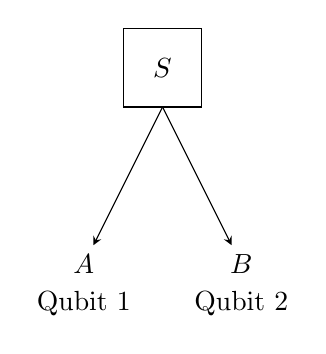
\begin{tikzpicture}
				\node (A) at (1, 0) {\(  B \)};
				\node (B) at (-1, 0) {\( A \) }; 
				\draw (-0.5, 2) rectangle node{\( S \) } (0.5, 3);
				\draw[-stealth] (0, 2) -- (A); 
				\draw[-stealth] (0, 2) -- (B);
				\draw node at (1, -0.5) {Qubit 2};
				\draw node at (-1, -0.5) {Qubit 1};
			\end{tikzpicture}
		\end{center}
	\item Classically, if an observer were to say, measure the second qubit, then send an identical copy through 
		that channel, then Alice and Bob won't be able to tell at all that the state has been measured. 

		However, if the system was quantum, this measurement is now impossible. 
	\item The proof of this is called the No cloning theorem, whose proof is below: 

		\begin{proof}
			Suppose we have an unknown state   \( \ket*{\phi} = \alpha \ket*{0} + \beta \ket*{1} \).  Now suppose 
			there is a \( U_{cl} \) (a "cloning matrix") which can clone \( \ket*{\phi} \). That is:
			\[
			\ket*{\phi}\ket*{0} \mapsto \ket*{\phi}\ket*{\phi} = \alpha^2 \ket*{00} 
			+ \beta \alpha \ket*{10} + \alpha \beta \ket*{01} + \beta^2 \ket*{11}
			\] 
			But if we do this on the initial state \( \ket*{\phi} \) : 
			\[
				(\alpha \ket*{0} + \beta \ket*{1}) \ket*{0} \mapsto \alpha \ket*{00} +\beta \ket*{11}
			\] 
			\comment{We are cloning this exactly based on what we want: we clone the information of the second 
				qubit onto the first qubit, but we see that even if we could "copy", we don't get the desired 
			product state.} 

			But this is not equal to the copied state that we should expect. Therefore, no such \( U_{cl} \) 
			can exist.
		\end{proof}
\end{itemize}
\subsection{Quantum Algorithms}
\begin{itemize}
	\item The Deutsch-Josza is a \textit{promise problem}: we are given a function \( f(x) \), and 
		it's one of two types: 
		\begin{itemize}
			\item \( f(x) \) is either constant for all \( x \) : it is either always 0 or always 1.
			\item \( f(x) \) is balanced: it is 0 half the time, \( f(x)  \) is 1 half the time. 
		\end{itemize}

		More generally, we can write \( f: \{0, 1\} ^{n} \mapsto \{0, 1\}  \), and we ask whether \( f \) is 
		constant or balanced. 
	\item For a function on \( n \) bits, this implies that the total domain space is of size \( 2^{n} \). We need to 
		measure a little more than half, or \( 2^{n} / 2 + 1 = 2^{n - 1} + 1 \) measurements in order to determine 
		the identity of \( f \).

		Quantumly, we only need a single measurement!
	\item The quantum circuit is as follows:
		\begin{center}
			\begin{quantikz}[slice all, slice titles = $\ket{\psi_\col}$ ]
				\lstick{\( \ket*{0}^{\otimes n} \)} \slice{\( \ket*{\psi_0} \) } & \gate{H^{\otimes n}} & \gate[2]{ U_f } & \gate{H^{\otimes n}} & \\
				\lstick{\( \ket*{1} \) } & \gate{H} & & & 
			\end{quantikz}
		\end{center}
		Initially, the state is in \( \ket*{\psi_0} = \ket*{0}^{\otimes n} \ket*{1} \). Then, after passing through 
		both Hadamard gates, we have: 
		\[
		\ket*{\psi_1} = \frac{1}{\sqrt{2}}\sum_x \ket*{x} \otimes \frac{1}{\sqrt{2} }(\ket*{0} - \ket*{1})
		\] 
		To explain what's happening here, here's a convenient way to denote \( H \) : 
		\[
		H = \frac{1}{\sqrt{2} }\sum_{x, y \in \{0, 1\} } (-1)^{xy}\ket*{y}\bra*{x}
		\] 
		(check for yourself that this does indeed generate the correct Hadamard matrix). Therefore, the general 
		\( n \)-qubit Hadamard gate \( H^{\otimes n} \) :
		\[
		H^{\otimes n} = \frac{1}{\sqrt{2^{n}} }\sum_{x, y \in \{0, 1\} ^{n}}(-1)^{x \cdot y}\ket*{y}\bra*{x}
		\] 
		Therefore, we can write:
		\[
			\ket*{\psi_1} = H^{\otimes n}\ket*{0^{\otimes n}} \otimes \frac{1}{\sqrt{2} }(\ket*{0} -\ket*{1})
			= \frac{1}{\sqrt{2^{n}} }\sum_x \ket*{x} \otimes \frac{1}{\sqrt{2} }(\ket*{0} - \ket*{1})
		\] 
	\item Now we send \( \ket*{\psi_1} \) through \( U_f \). What it does is it sends \( \ket*{y} \) 
		to \( \ket*{y \oplus f(x)} \). If \( y = 0 \), then we just output \( f(x) \), and if \( y = 1 \), thne 
		we output the \textit{complement} of \( f(x) \), since if \( f(x) = 1 \) then the addition modulo 2 
		would return us 0, and vice versa. Therefore, we can write \( \ket*{\psi_2} \) as: 
		\[
			\ket*{\psi_2} = \frac{1}{\sqrt{2^{n}} }\sum_x \ket*{x }\otimes \frac{1}{\sqrt{2} }
			(\ket*{f(x)} - \ket*{\overline{f(x)}})
		\] 
		If \( f(x) = 0 \), then the ancilla (the last qubit) is \( \ket*{0} - \ket*{1} \), and if \( f(x) = 1 \), 
		then the ancilla is  \( \ket*{1} - \ket*{0} = -(\ket*{0} - \ket*{1}) \). So in general, the ancilla is 
		\( (-1)^{f(x)}(\ket*{0} - \ket*{1})  \). Therefore, we can write:
		\[
		\ket*{\psi_2} = \frac{1}{\sqrt{2^{n}} } \sum_x (-1)^{f(x)}\ket*{x} \otimes \frac{1}{\sqrt{2} }(\ket*{0} - \ket*{1})
		\] 
		\comment{We can write \( (-1)^{f(x)} \) because when \( f(x) = 0 \) then \( (-1)^{f(x)} = 1 \), which doesn't
		change the product at all, but it changes when \( f(x) = 1 \), which is what we want.}
	\item Finally, we act \( H^{\otimes n} \) on the data register. Note that \( H^{\otimes n}\ket*{x} = 
		\sum_y (-1)^{xy}\ket*{y}\), so this gives us:
		\[
		\ket*{\psi_3} = \frac{1}{\sqrt{2^{n}} }\sum_y\sum_x (-1)^{f(x) + (x \cdot y)}\ket*{y} \otimes 
		\frac{1}{\sqrt{2} }(\ket*{0} - \ket*{1})
		\] 
	\item Now we measure all \( n \) qubits. If \( f(x) \) is constant, 
\end{itemize}

	\section{Lecture 6}
\subsection{Clarification on BIBO Stability}
\begin{itemize}
	\item When we say a "bounded" signal, we mean that the amplitude of the signal is bounded at all times:
		\[
		|x(t)| < \infty \ \forall t \in \R
		\] 
		The same definition follows for discrete-time signals. 
	\item For LTI systems, we call the system BIBO stable if and only if its impulse \( h(t) \) is absolutely 
		integrable:
		\[
		\int_{-\infty}^{\infty} |h(t)| \diff t < \infty
		\] 
\end{itemize}
\subsection{Cross-Correlation}
\begin{itemize}
	\item The cross correlation between two signals \( r_{xy}(t) = r_{yx}(-t) \). To show this explicitly, we 
		look at the cross-correlation equation:
		\begin{align*}
			r_{xy}(t) &= \int_{-\infty}^{\infty} x(\tau)y(t + \tau) \diff \tau \\
			r_{yx}(t) &= \int_{-\infty}^{\infty} y(\tau) x(t + \tau) \diff \tau  
	\end{align*} 
	But for the second equation, we can define a \( \tau' = t + \tau\), so then we get: 
	\[
	r_{yx}(t) = \int_{-\infty}^{\infty} y(\tau' - t)x(\tau') \diff \tau' = \int_{-\infty}^{\infty} 
	x(\tau') y(-t + \tau') \diff \tau'
	\] 
	This looks like the first equation except we have \( -t \) instead of \( t \). Therefore, we have 
	\( r_{xy}(t) = r_{yx}(-t) \). The same works for discrete time: \( r_{xy}[n] = r_{yx}[-n] \). 
\end{itemize}

\subsection{More Convolution Properties} 
\begin{itemize}
	\item \textbf{Differentiation property:} Given \( y(t) = x(t) * h(t) \), then:
		\[
			\dv{t} y(t) = x(t) * \dv{h(t)}{t} = \dv{x(t)}{t} * h(t)
		\] 
	\item \textbf{Intergration Property:} Given \( y(t) = x(t) * h(t) \), we have:
		\[
		\int_{-\infty}^{t'} y(t) \diff  t = x(t) * \int_{-\infty}^{t'} h(\tau)\diff \tau 
		\] 
\end{itemize}
\subsection{Fourier Transform} 
\begin{itemize}
	\item The fourier transform came from the study of the heat equation, written as:
		\[
			c \rho \pdv{t} u(x, y, z, t) = k \left( \pdv[2]{x} + \pdv[2]{y} + \pdv[2]{z} \right) 
			u(x, y, z, t)
		\] 
		Fourier then claimed that the solution can be expanded in a series of sines with multiples of the variable. 
		In other word,s the solution is of the form:
		\[
		f(x) = \frac{1}{2a_0} + (a_1 \sin(x) + b_2 \cos(x)) + (a_2\sin(2x) + b_2\cos(2x)) + \cdots 
		\] 
	\item Recall the frequency response of an LTI system:
		\begin{center}
			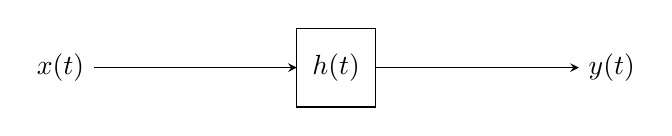
\begin{tikzpicture}
				\node (A) at (-3, 0) {\( x(t) \) };
				\node (B) at (4, 0) {\( y(t) \) };
				\draw[-stealth] (A) -- (0, 0);
				\draw (0, -0.5) rectangle node {\( h(t) \) } (1, 0.5);
				\draw[-stealth] (1, 0) -- (B);
			\end{tikzpicture}
		\end{center}
		Recall that we can characterize \( y(t) \) via a convolution: 
		\[
		y(t) = \int_{-\infty}^{\infty} x(\tau) h(t - \tau) \diff  \tau 
		\] 
		If we do this with our input \( e^{j 2 \pi ft} \), then we get:
		\[
		y(t) = H(f) e^{j 2 \pi ft} = H(\omega) e^{j \omega t }
		\] 
		Here, \( H(\omega) \) is defined to be the Fourier transfrm of the impusle response \( h(t) \):
		\[
			H(\omega) = \int_{-\infty}^{\infty} e^{- j \omega t} h(t) \diff t 
		\] 
		Alternatively, written in frequency language:
		\[
		H(f) = \int_{-\infty}^{\infty} e^{-j 2 \pi ft}h(t) \diff t 
		\] 
	\item Formally, the Fourier transform is defined as:
		\[
		H(f) \equiv \mathcal F \{h(t)\} \equiv \int_{-\infty}^{\infty} h(t) e^{-j 2\pi ft }\diff  t 
		\] 
		This transforms the signal \( h(t)  \) from the time domain into the frequency domain. The reason for this 
		is becuase the Fourier transform is a definite integral, which kills off any \( t \) dependence entirely. 
		In terms of angular frequency, we have:
		\[
		H(\omega) \equiv \mathcal F \{h(t)\} = \int_{-\infty}^{\infty} h(t) e^{-j \omega t}\diff t 
		\] 
	\item The inverse Fourier transform is:
		\[
			h(t) = \mathcal F^{-1} \{H(f)\} = \int_{-\infty}^{\infty} H(f) e^{j 2\pi ft}\diff  f 
		\]
		Since the Fourier transform takes objects from the time domain to the frequency domain, the inverse 
		Fourier transform takes things from the frequency domain to the time domain. 

		In terms of angular frequency, we have:
		\[
		h(t) = \mathcal F^{-1} \{H(\omega)\} = \frac{1}{2\pi}\int_{-\infty}^{\infty} H(\omega) 
		e^{j \omega t}\diff \omega 
		\] 
		This is also sometimes called the "synthesis equation", since we basically create \(  x(t) \) out of 
		\( H(\omega) \). 
	\item We can also provably show that the Inverse fourier transform does indeed invert the Fourier transform, 
		albeit with a lot of algebra. See lecture slides for the full derivation.  
	\end{itemize}

\end{document}
